% Template for PLoS
% Version 2.0 July 2014
%
% To compile to pdf, run:
% latex plos.template
% bibtex plos.template
% latex plos.template
% latex plos.template
% dvipdf plos.template
%
% % % % % % % % % % % % % % % % % % % % % %
%
% -- IMPORTANT NOTE
%
% Be advised that this is merely a template
% designed to facilitate accurate translation of manuscript content
% into our production files.
%
% This template contains extensive comments intended
% to minimize problems and delays during our production
% process. Please follow the template
% whenever possible.
%
% % % % % % % % % % % % % % % % % % % % % % %
%
% Once your paper is accepted for publication and enters production,
% PLEASE REMOVE ALL TRACKED CHANGES in this file and leave only
% the final text of your manuscript.
%
% DO NOT ADD EXTRA PACKAGES TO THIS TEMPLATE unless absolutely necessary.
% Packages included in this template are intentionally
% limited and basic in order to reduce the possibility
% of issues during our production process.
%
% % % % % % % % % % % % % % % % % % % % % % %
%
% -- FIGURES AND TABLES
%
% DO NOT INCLUDE GRAPHICS IN YOUR MANUSCRIPT
% - Figures should be uploaded separately from your manuscript file.
% - Figures generated using LaTeX should be extracted and removed from the PDF before submission.
% - Figures containing multiple panels/subfigures must be combined into one image file before submission.
% See http://www.plosone.org/static/figureGuidelines for PLOS figure guidelines.
%
% Tables should be cell-based and may not contain:
% - tabs/spacing/line breaks within cells to alter layout
% - vertically-merged cells (no tabular environments within tabular environments, do not use \multirow)
% - colors, shading, or graphic objects
% See http://www.plosone.org/static/figureGuidelines#tables for table guidelines.
%
% For sideways tables, use the {rotating} package and use \begin{sidewaystable} instead of \begin{table} in the appropriate section. PLOS guidelines do not accomodate sideways figures.
%
% % % % % % % % % % % % % % % % % % % % % % % %
%
% -- EQUATIONS, MATH SYMBOLS, SUBSCRIPTS, AND SUPERSCRIPTS
%
% IMPORTANT
% Below are a few tips to help format your equations and other special characters according to our specifications. For more tips to help reduce the possibility of formatting errors during conversion, please see our LaTeX guidelines at http://www.plosone.org/static/latexGuidelines
%
% Please be sure to include all portions of an equation in the math environment, and for any superscripts or subscripts also include the base number/text. For example, use $mathrm{mm}^2$ instead of mm$^2$ (do not use \textsuperscript command).
%
% DO NOT USE the \rm command to render mathmode characters in roman font, instead use $\mathrm{}$
% For bolding characters in mathmode, please use $\mathbf{}$
%
% Please add line breaks to long equations when possible in order to fit our 2-column layout.
%
% For inline equations, please do not include punctuation within the math environment unless this is part of the equation.
%
% For spaces within the math environment please use the \; or \: commands, even within \text{} (do not use smaller spacing as this does not convert well).
%
%
% % % % % % % % % % % % % % % % % % % % % % % %



\documentclass[10pt]{article}

% amsmath package, useful for mathematical formulas
\usepackage{amsmath}
% amssymb package, useful for mathematical symbols
\usepackage{amssymb}

% cite package, to clean up citations in the main text. Do not remove.
\usepackage{cite}

\usepackage{hyperref}

% line numbers
\usepackage{lineno}

% ligatures disabled
\usepackage{microtype}
\DisableLigatures[f]{encoding = *, family = * }

% rotating package for sideways tables
%\usepackage{rotating}

% If you wish to include algorithms, please use one of the packages below. Also, please see the algorithm section of our LaTeX guidelines (http://www.plosone.org/static/latexGuidelines) for important information about required formatting.
%\usepackage{algorithmic}
%\usepackage{algorithmicx}

% Use doublespacing - comment out for single spacing
%\usepackage{setspace}
%\doublespacing


% Text layout
\topmargin 0.0cm
\oddsidemargin 0.5cm
\evensidemargin 0.5cm
\textwidth 16cm
\textheight 21cm

% Bold the 'Figure #' in the caption and separate it with a period
% Captions will be left justified
\usepackage[labelfont=bf,labelsep=period,justification=raggedright]{caption}

% Use the PLoS provided BiBTeX style
\bibliographystyle{plos2009}

% Remove brackets from numbering in List of References
\makeatletter
\renewcommand{\@biblabel}[1]{\quad#1.}
\makeatother


% Leave date blank
\date{}

\pagestyle{myheadings}

%% Include all macros below. Please limit the use of macros.

%% END MACROS SECTION


\begin{document}


% Title must be 150 characters or less
\begin{flushleft}
{\Large
\textbf{Plant Photosynthetic Heterogeneity Reveals New ...}
}
% Insert Author names, affiliations and corresponding author email.
\\
Oliver L Tessmer$^{1}$,
Jeffrey A Cruz$^{2,3}$,
Linda J Savage$^{2}$,
David M Kramer$^{2,3,\ast}$,
Jin Chen$^{1,2,\ast}$
\\
\bf{1} Department of Computer Science and Engineering, Michigan State University, East Lansing, MI, USA
\\
\bf{2} Department of Energy Plant Research Laboratory, Michigan State University, East Lansing, MI, USA
\\
\bf{3} Department of Department of Biochemistry and Molecular Biology, Michigan State University, East Lansing, MI, USA
\\
$\ast$ E-mail: jinchen@msu.edu, kramerd8@msu.edu
\end{flushleft}

% Please keep the abstract between 250 and 300 words
\section*{Abstract}

Photosynthetic heterogeneity is a universal phenomenon among plants...

\section*{Author Summary}

Photosynthetic heterogeneity is a universal phenomenon among plants...

\section*{Introduction}


%[Phenotyping]
Using sunlight, water and $CO_2$, plants produce sugars and release $O_2$ with photosynthesis \cite{kramer2011importance}. The process involves the formation of high energy intermediates capable of generating reactive oxygen species. The photosynthetic apparatus, chloroplast and surrounding leaf tissue is inherently susceptible to oxidative damage, especially under stress conditions when the supply of light energy exceeds the capacity to utilize it \cite{asada1996radical,durrant1990characterisation}. Plants have evolved a number of mechanisms, such as photosynthetic apparatus damage and repair \cite{melis1999photosystem}, to dissipate excess light energy to minimize the potential for damage at the expense of photosynthetic efficiency \cite{adams2006energy,rochaix2014regulation}. However, these mechanisms are sensitive to leaf development and thus may change from one leave tissue to another, resulting in heterogenous photosynthetic patterns (see Figure \ref{fig:heterogeneityexample}). These patterns also vary with the position, size and growth rate of leaves, since leaves at the same node is unique in age. By integrating plant morphological and physiological features, measuring plant photosynthetic heterogeneity aids interpretation of the sophisticated photosynthesis mechanism, particularly important for plant primary productivity estimation and modeling \cite{meng2007spatial}.

%Advanced technologies in high-throughput plant photosynthetic phenotyping (the Dynamic Environment Photosynthesis Imager, or DEPI) have been developed \cite{cruz2014depi,houle2010phenomics}. These systems generate huge amount of images of plant photosynthesis that can be used to quantify photosynthetic behavior in genetically diverse populations, leading to better understanding of the underlying mechanisms that control the photosynthetic properties \cite{fiorani2013future,rascher2011non}, enabling to measure variability in various photosynthetic parameters at high resolution across leaves.

%The model of spatial heterogeneity of the photosynthetic properties may reveal $CO_2$ intake capability, stomatal conductance and tolerance level to environmental changes of leaf tissues at different developmental stages.

%photosynthetic heterogeneity refers to a plant comprising multiple regions, a significant amount of which have different photosynthesis properties, %. %For example, under full sunlight photosynthesis usually captures at most only of available energy (bonner1962upper, von1981some, kramer2011importance).

Heterogeneity is a concept relating to the uniformity in a substance. The granularity of photosynthetic heterogeneity ranges from cells to tissues, leaves, and even the whole plant. While in-leaf variability in photosynthetic activity has been well-studied for the understanding of the effects of stomatal conductance \cite{Buckley1997,Cheeseman1991}, recent works show that photosynthetic capacity may decline with vertical gradient and leaf age \cite{chen2008effect,Kitajima2002}, indicating that leaf-based photosynthetic heterogeneity is a key towards the understanding of plant photosynthesis.

The leaf heterogeneity in photosynthesis was firstly been studied  with a simulation model \cite{chen2008effect}. Due to the lack of high-throughput phenotyping technologies, the authors determined the effects of biochemical variability via the Farquhar model incorporating defined degrees of spatial variability of its parameters. The Farquhar model is a mechanistic, biochemical model widely used to describe steady-state $CO_2$ assimilation in leaves \cite{farquhar2001models,sharkey1985o2}. Spatial heterogeneity in photosynthesis was found to have an effect on the ability of the Farquhar model to accurately characterize photosynthesis at the leaf level \cite{chen2008effect}.

Recently, with the advent of advanced technologies of biomedical imaging, directly measuring heterogeneity has recently assumed new importance {\cite{cruz2014depi,tiihonen1996cerebral,wieneke1999non,wang2000}. The rapid development of lighting and imaging techniques enables real-time non-invasive monitoring of photosynthesis \cite{cruz2014depi,houle2010phenomics}, resulting in vast amount of images of plant photosynthesis \cite{wituszynska2013multivariable}. These images can be used to quantify photosynthetic behavior in genetically diverse populations, enabling to measure variability of photosynthetic parameters at high resolution across leaves, leading to better understanding of the underlying mechanisms that control the photosynthetic properties \cite{fiorani2013future,rascher2011non}.

%\begin{figure}[!t]
%\begin{center}
%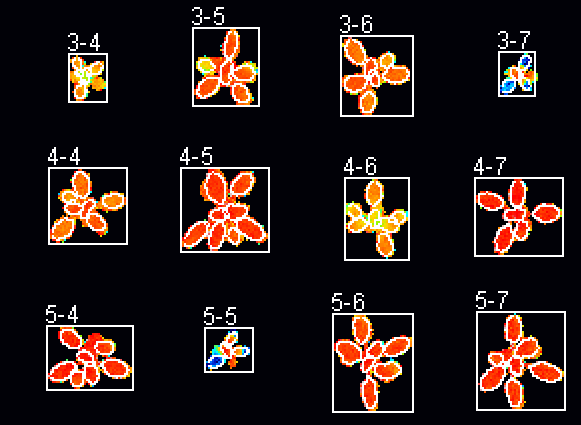
\includegraphics[width=2in]{preprocessing.png}
%\caption{\small Examples of leaf-level photosynthetic heterogeneity.}
%\end{center}\label{fig:heterogeneityexample}
%\end{figure}

In order to measure leaf-based photosynthetic variability in a large-scale phenotyping experiment, in which hundreds of plants are screened simultaneously, it is required to automatically segment each leaf from top-view images, and then measure the variations of photosynthesis parameters across leaves.
Photosynthesis images are false-color images, where the light intensity of every pixel is proportional to photosynthetic efficiency \cite{toet1996new} (see Figure \ref{fig:heterogeneityexample}). Differences between individual leaves with similar photosynthetic efficiency can be subtle, making the boundaries between them difficult to define and creating a significant challenge for subsequent shape analysis. The difficulty even arises when individual leaves overlap and occlude one another in these false-color images.
%challenges in heterogeneity measure
...

%We have developed a new leaf segmentation approach called leafPH to identify leaves from photosynthesis images...

In this paper, we present a new computational framework called leafPH and use the tool to minitor the leaf-level photosynthesis heterogeneity of more than 100 Arabidopsis chloroplast mutant strains, each with at least four replicates. The mutant screen analysis reveals that ...



%---------------------------

\section*{Results}

In plants, photosynthetic heterogeneity refers to a plant comprising multiple regions, many of which have different photosynthesis properties, potentially because of vastly different leaf developmental stage and tolerance level to environmental changes. By developing an efficient plant photosynthetic heterogeneity measure leafPH and applying it on more than 100 Arabidopsis chloroplast mutant strains, we show that ...

\subsection*{Framework of leafPH} \label{sec:leafPH}

We first introduce the framework of leafPH which consists two major modules: leaf alignment and tracking and heterogeneity measurement. The architecture of the application is shown in Figure ??. First of all, we have developed the leaf alignment algorithm \cite{yin2014}. This paper focus on the measure of 

Comparing with the existing heterogeneity approaches, our method is novel in the following ways:

1.	leafPH relies on a novel leaf alignment and tracking method... %, which considers plant-specific constraints including leaf shape similarity and symmetry. By taking the biological knowledge about the shapes of any possible leaf into account, we add flexibility to the model to fit to all the general leaves. Specifically, for leaf boundary identification, we develop a leaf symmetry based curve fitting model to define the initial shape of a leaf, and develop a plant layout based approach to define leaf tips and orientation, therefore defining the leaf initial position.  Note that since leaf is assumed to be symmetric, curve fitting could converge without large amount of training.

2. leafPH models heterogeneity of photosynthesis with size, position and growth rate...

3. leafPH refers to the differences between individual leaf photosynthesis and the pooled photosynthesis across all the leaves, with the weights being those used in the pooling method. With leafPH, transient regional variation events that do not affect the whole plant photosynthesis, can be easily discovered.

\subsubsection*{Basic heterogeneity measurement}

Let $T = \{T_{1}, T_{1}, \ldots\, T_{n}\}$ be the set of effect estimates of a plant $p$ with $n$ leaves. 
%
In each study $T_i$, let $u_i$ and $u_p$ be the averaged photosynthesis values of leaf $l_i$ and the averaged photosynthesis values of whole plant $p$, and $std(l_i)$ and $std(p)$ be the population standard deviations, respectively. Under the assumption of normal distribution and homoscedasticity, the effect estimate $T_i$ is the standardized mean difference \cite{hedges1998fixed}, which can be estimated by %$T_{i} = c(l_i) (mean(l_i)-mean(p))/S(l_i,p)$ ,

\begin{equation}\label{eq:effectestimate}
T_{i} =  \frac{c(l_i)\left(\mu(l_i)-\mu(p)\right)}{S(l_i,p)}
\end{equation}

\noindent where $mean(.)$ is the averaged photosynthesis value, $c(l_i)$ is a correction factor for the positive bias suffered by the standardized mean difference with small sample sizes, which can be estimated by $c(l_i) = 1-3/(4(|l_i|-1)-1)$ \cite{hedge1985statistical}. Such adjustment will reduce the effect estimate of small leaves that only have a few pixels, and thus increase the robustness of the heterogeneity model.
%
%According to the equation of $c(L_i, L_j)$, $c(L_i, L_j)$ is close to 1 for large leaves with many pixels, otherwise it is close to 0, down-weighing the value of heterogeneity. 
%
The pooled estimate of the within-group standard deviation $S(l_i, p)$ can be computed with \cite{hedges1998fixed}:

\begin{equation}\label{eq:S}
S(l_i, p) = \sqrt{\frac{(|l_i|-1)std^2(l_i)+(|p|-1)std^2(p)}{|l_i|+|p|-2}}
\end{equation}

\noindent where $std^2(.)$ is the standard variance and $|.|$ is the total number of pixels.

%The sample variance of $T_{ij}$ is estimated using Equation \ref{eq:ST} \cite{hedges1998fixed}.
%
%\begin{equation}\label{eq:ST}
%ST_{ij} = \frac{|L_i|+|L_j|}{|L_i||L_j|}+\frac{T_{ij}^2}{2(|L_i|+|L_j|)}
%\end{equation}

Second, we apply Cochran's Q-test statistic for determining whether there is true leaf-based photosynthetic heterogeneity among the leaves:
%
\begin{equation}\label{eq:Q}
%Q=\sum_{i=1}^n \frac{\left(T_i-mean(T)\right)^2}{\tau^2}
Q=\sum_{i=1}^n w_i\left(T_i-mean(T)\right)^2
\end{equation}

\noindent where $n$ is the number of leaves of plant $p$, and $w_i=1/(\tau^2+\delta_i^2)$. Note that we ignored the computation of the sampling variance of the effect estimate $\delta_i^2$, since we count the photosynthesis value of every pixel in the test.
%
The between-study variance $\tau^2$ is the parameter in the statistical model that mainly represents the true heterogeneity among the true effects of the studies. Therefore, a good procedure for determining whether there is true heterogeneity among all leaves of a plant should be positively correlated with $\tau^2$. At the same time, it should not be affected by the number of leaves, and should be scale-free in order to be comparable among different plants.  

We estimate $\tau^2$ using an estimator based on the method of moments \cite{dersimonian1986meta}:

\begin{equation}\label{eq:tau}
\tau^2 = \left\{\begin{matrix}
 \frac{\widetilde{Q}-(n-1)}{\sum \widetilde{w_{i}}-\frac{\sum \widetilde{w_{i}}^2}{\sum \widetilde{w_{i}}}} & \widetilde{Q}>|T|+1\\
 0 & else
\end{matrix}\right.
\end{equation}

\noindent where $\widetilde{Q}$ and $\widetilde{w_{ij}}$ are the results of Q test of fixed effect estimate and the corresponding weight.

\begin{equation}\label{eq:weight}
\widetilde{w_{ij}}=[Pos(L_i)\neq  Pos(L_j)] \times \frac{min(|L_i|, |L_j|)}{(ST^2_{ij}+c) \sum L}
\end{equation}

One problem with the Q test is that its statistical power depends 

\subsubsection*{Heterogeneity measurement of position, size and growth of leaves}


\subsection*{leafPH on Arabidopsis data}

The L'Abbe plot can be used to visually explore the inconsistency of leaf-based photosynthesis.

\subsection*{leafPH on synthetic data}

% You may title this section "Methods" or "Models".
% "Models" is not a valid title for PLoS ONE authors. However, PLoS ONE
% authors may use "Analysis"
\section*{Materials and Methods}

\subsection*{Data Acquisition and Preprocessing}

In the photosynthesis phenotyping experiment, hundreds of Arabidopsis thaliana plants (wild type, genetic variations with gene knockout or over-expression, ecotypes, etc) were grown side-by-side under three different light conditions (constant, sinusoid, fluctuate), for in total three days.
%
Top-view fluorescence images were collected every 15 minutes in order to observe the photosynthesis activity of all of the plants simultaneously. Each fluorescence image is a grey-scale image with a resolution of 1M pixels at 12-bit intensity.

To accurately capture the photosynthesis activities of plants from fluorescence images, a image segment method is applied to remove the background, identify every piece of leaf~\cite{yin2014}, measure the intensity of pixels on leaves, and finally convert the intensity values to the measure of four kinds of photosynthesis parameters.
%
The extracted measurements of photosynthesis parameters are presented in the form of multi-dimensional time-series, one dimension for every photosynthesis parameter.
%
Figure 1 shows that the measurements of a photosynthesis parameter $\Phi_2$ at one time point are quite different for the leaves of the same plant  (i.e. plant no. 3-7 and 5-5).

\subsection*{Leaf alignment and tracking}

For completeness, we introduce the leaf alignment and tracking approach...

\subsection*{Heterogeneity Test}

Cochran's Q-test is the classical measure of heterogeneity \cite{conover1999Practical}. In leaf-based photosynthetic heterogeneity, Q is calculated as the weighted sum of squared differences between the photosynthesis value of a individual leaf and the pooled photosynthesis value across all leaves with the weights being those used in the pooling method. The distribution of Q is a chi-square statistic with $k-1$ degrees of freedom, where $k$ is the number of leaves. Cochran's Q-test has been widely used in biomedical studies. For example, heterogeneity in the aggressiveness of tumor cell populations has been adopted as an essential feature in predicting treatment success \cite{OSullivan2003}. However, due to the nature of plant, leaf-based photosynthetic heterogeneity often includes a small number of leaves, and thus the power of the Q-test in such circumstances is low \cite{higgins2003measuring, gavaghan2000evaluation}.
%
%Conversely, Q has too much power as a test of heterogeneity if the number of leaves is large \cite{higgins2003measuring}.

%An additional test is provided with the odds ratio meta-analysis \cite{breslow1987statistical}. It is arguably not possible to examine the null hypothesis that all studies are evaluating the same effect, by considering the only the summary data from the studies: The heterogeneity test results should be considered alongside a qualitative assessment of the combinability of studies in a systematic review.

The $I^2$ statistic describes the percentage of variation across studies that is due to heterogeneity rather than chance \cite{higgins2002quantifying,higgins2003measuring}. $I^2$ can be calculated  as $I^2 = (Q - df)/Q$, where Q is Cochran's Q-test heterogeneity statistic and $df$ is the degrees of freedom. A negative value  indicates no observed heterogeneity, and larger values show increasing heterogeneity. $I^2$ is an intuitive and simple expression of the inconsistency. $I^2$ of leaf-based photosynthetic heterogeneity does not inherently depend upon the number of leaves, so that $I^2$ values of different plants become comparable. A confidence interval for $I^2$ is constructed using either the iterative non-central chi-squared distribution method \cite{hedges2001power} or the test-based method \cite{higgins2002quantifying}.

Based on Cochran's Q-test and the $I^2$ statistic, we develop a new approach that quantifies the effect of heterogeneity of photosynthesis across leaves of the same plant, and compare the degree of inconsistency among mutant strains in varying environmental conditions (see Section~\ref{sec:leafPH}). The challenges of this work include the leaf alignment and the new heterogeneity measure that takes leaf position, size and growth into consideration.

%To measure leaf-based photosynthetic variability in a large-scale phenotyping experiment, in which hundreds of plants are monitored in real time, it is naturally required to identify each leaf from top-view photosynthesis images automatically. However, leaf identification is a difficult task, in that 1) all the leaves are very similar in appearance especially for model plant Arabidopsis; 2) leaf features are much fewer than the well-studied face recognition problem; and 3) leaves may overlapped with each other that makes the problem more complicated. In short, there are two challenging computational problems. First, how to separate overlapped leaves in photosynthesis images where the leaf boundaries are obscure. Second, how to recognize incomplete leafs due to occlusion. Alternatively, approximation approaches can be used to estimate the leaf-based photosynthetic heterogeneity, including distribution based, region based and pixel based approaches. While these approximation approaches are easier to model, their performance may be reduced.

% Results and Discussion can be combined.


\section*{Discussion}

A consensus view of the data is that the photosynthesis ability of a plant is not uniform across the whole area (Charles 2008, Meng 2007).
%
The photosynthetic properties of plants can vary dramatically across cells, tissues, and organs~\cite{}, reflecting differences in development, stress responses, regulation of processes such as stomatal conductance~\cite{}, photodamage~\cite{}, and storage of photosynthate~\cite{} and contribute substantially to productivity~\cite{}.

For example, we observed that the acclimation of photosynthesis in response to cold temperatures appears to be more rapid and robust in younger or emerging than older leaves, and ecotypes isolated from different latitudes show distinct heterogeneity patterns, implying that these responses are important for adaptation of photosynthesis to fluctuating temperatures.
%
In other cases, exposure of plants to fluctuating light resulted in loss of photosynthetic capacity or increased photoinhibition in specific sets of leaves or leaf sectors. In many cases, older leaves are preferentially affected, suggesting that resources for maintenance or acclimation responses are preferentially directed to younger leaves. However, we have also identified mutant lines where younger leaves are preferentially affected, which presumably affect the development of photosynthetic robustness.

In order to systematically study the leaf level photosynthesis phenotypes, especially in a high-throughput screen manner, we developed a novel computational tool to automatically conduct statistical analysis on leaf based photosynthesis.


% Do NOT remove this, even if you are not including acknowledgments.

\section*{Acknowledgments}


\section*{References}

% Either type in your references using
% \begin{thebibliography}{}
% \bibitem{}
% Text
% \end{thebibliography}
%
% OR
%
% Compile your BiBTeX database using our plos2009.bst
% style file and paste the contents of your .bbl file
% here.
%

\section*{Figure Legends}
% This section is for figure legends only, do not include
% graphics in your manuscript file.
%
%\begin{figure}
%\caption{
%{\bf Bold the first sentence.}  Rest of figure caption.
%}
%\label{Figure_label}
%\end{figure}


\section*{Tables}
%
% See introductory notes if you wish to include sideways tables.
%
% NOTE: Please look over our table guidelines at http://www.plosone.org/static/figureGuidelines#tables to make sure that your tables meet our requirements. Certain types of spacing, cell merging, and other formatting tricks may have unintended results and will be returned for revision.
%
%\begin{table}[!ht]
%\caption{
%\bf{Table title}}
%\begin{tabular}{|c|c|c|}
%table information
%\end{tabular}
%\begin{flushleft}Table caption
%\end{flushleft}
%\label{tab:label}
% \end{table}

\section*{Supporting Information Legends}
%
% Please enter your Supporting Information captions below in the following format:
%\item{\bf Figure SX. Enter mandatory title here.} Enter optional descriptive information here.
%
%\begin{description}
%\item {\bf}
%\item {\bf}
%\end{description}

\small
\bibliographystyle{plain}
\bibliography{heterogeneity}

\end{document}

